\documentclass[main.tex]{subfile}

\begin{document}

\section{Offset Errors} 
\label{sec:nyquist_frequency}

\subsection{Null-Offset and Amplitude Error}
\label{sec:amplitude_error}

\begin{figure}[H]
	\begin{center}
		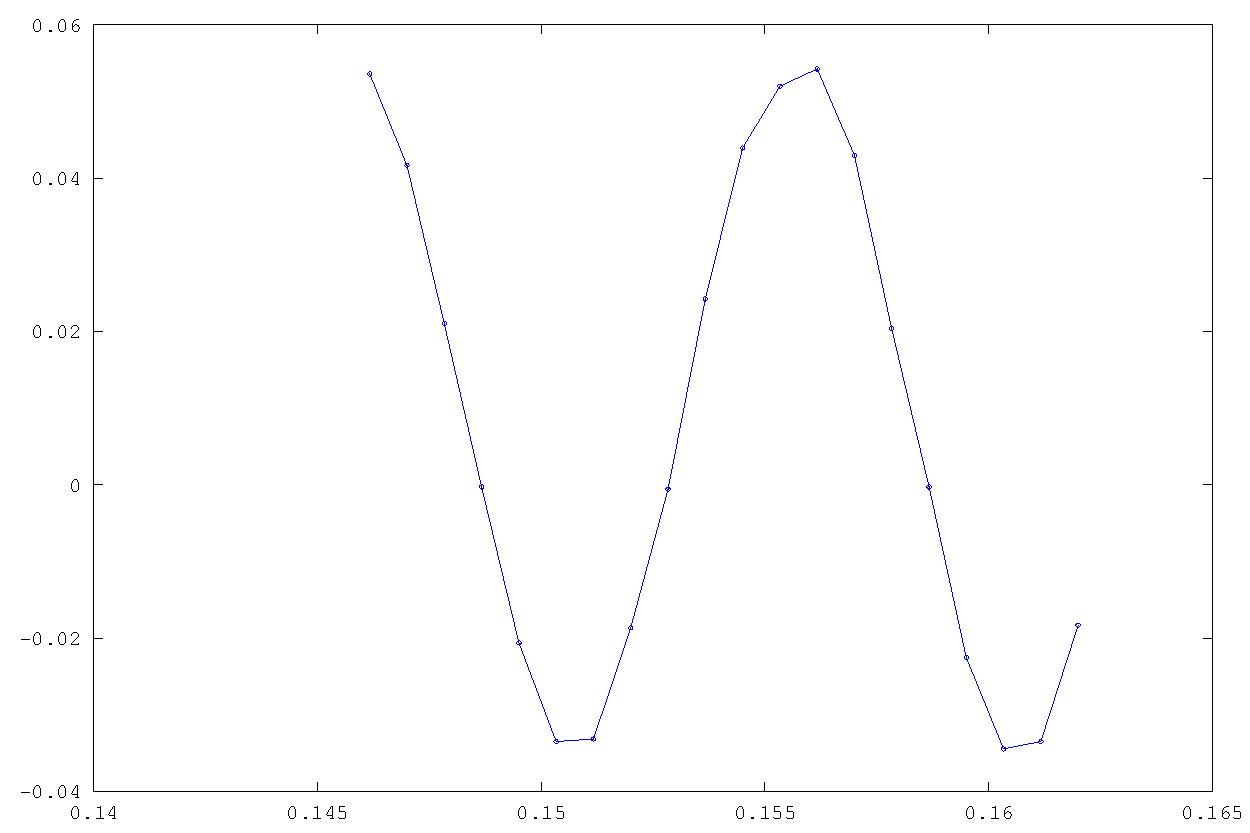
\includegraphics[width=\linewidth]{pt3}
	\end{center}
	\caption{Sinewave Sampled at $4\dem{kHz}$}
	\label{fig:4korig}
\end{figure}

As shown in \eqref{sampledWave} there are more potential errors present than
aliasing. Firstly there's potential to get the wrong $A_{pp}$ - the
peak-to-peak amplitude. To determine this amplitude error we use the maximum
absolute value in the sampled signal We then compare it to our expected
$A_{pp}$. 

For our experiment we use a sampling rate of $4\dem{kHz}$ (as shown in
\figref{4korig}) to avoid any aliasing error. \tabref{ampError} shows the
amplitude of the data gathered and the error compared to our expected $A_{pp} =
0.05$ of the data gathered. As seen the amplitude error does not fall within the
acceptable range.

\begin{table}[H]
  \begin{center}
    \caption{Collected data for Amplitude Error}
    \label{tab:ampError}
    \begin{tabular}{lll}
      \\ \toprule
      Maximum Abs. Value & \% Error  & Acceptable Amplitude Range
      \\ \midrule
      $0.054241$ & $8.48\%$ & $0.0495 - 0.0505$
      \\ \bottomrule
    \end{tabular}
  \end{center}
\end{table}

The second type of error we have is null-offset. Simply put this is the error in
the $y$ part of \eqref{sampledWave}. To calculate this we use the average value
of the sampled wave which - theoretically - should be $0$. The average value is
computed using $\frac{1}{t_2-t_1}\int_{t_1}^{t_2}{f(t) dt}$ where the integral
is evaluated using the trapezoidal method. We then find that the offset error of
the sine wave is $6.334e{-3}$.

To determine the exact sources of error more analysis would need to be
performed. However, with some common sense, we can make a rather educated guess.
First the amplitude error could come from the fact that the sampling frequency
is still to low to accurately depict the sampled wave. This is due to the fact
that the period of the sampling frequency is not at a low enough resolution to
capture the peaks of the sine wave. Thus a maximum amplitude seen by the sampled
data would be lower than that of the actual sine wave produced. 

Offset errors could be generated from improper grounding of the sinewave or the
sampling circuit. Also, limited sampling frequencies could produce an offset
error - as the offset is calculated using the amplitude of the sine wave. To
reduce these errors post data analysis could be performed to interpolate the
actual sine wave from the sampled data. Of course this would require a high
enough resolution such that the interpolation would accurately represent the
measured signal.

\subsection{Quantization Error}
\label{sec:quantization_error}

Because digital systems do not work with analog numbers directly but instead
quantize every number held within the computer's memory. Therefore data is lost
whenever you convert an analog signal to a digital one because each value being
converted into the system is "binned" or converted to the nearest floating point
number. Quantization is done relative to the range of input amplitudes of the
analog input port. That is the resolution of the quantization is shown in
\eqref{quantization}

\begin{align}
	Q = \frac{A_{pp}}{2^M}\label{eq:quantization}
\end{align}
where $Q$ is the resolution, $A_{pp}$ is the amplitude range of the bins we will
use, and $M$ is the number of bits that are used to represent the signal. The
resolution is the amplitude value per binary number used to represent the
signal.

If $A_{pp}$ does not cover the peak-to-peak amplitude of the wave we are
sampling then we will have a cut-off error. That is if the sampled wave has a
magnitude that is larger than the maximum value covered by our resolution then
the value will be binned to $2^M$ (that is all bits are $1$). If the resolution
is to small then the sampled wave will be restricted to small bounds within the
digital bins the sampled wave will appear to have an amplitude that is much
smaller than reality. This is similiar to plotting a function on a graph with a
y-axis scale that is much to large than necessary.

For our experiments we show both cases. First we test the small bin range case.
We do this by increasing the $A_{pp}$ of our generated signal from $0.1\dem{V}$
to $1\dem{V}$ while keeping the input range at $0.1\dem{V}$. The resulting graph
are truncated peaks as shown in \figref{smallQ};

\begin{figure}[H]
	\begin{center}
		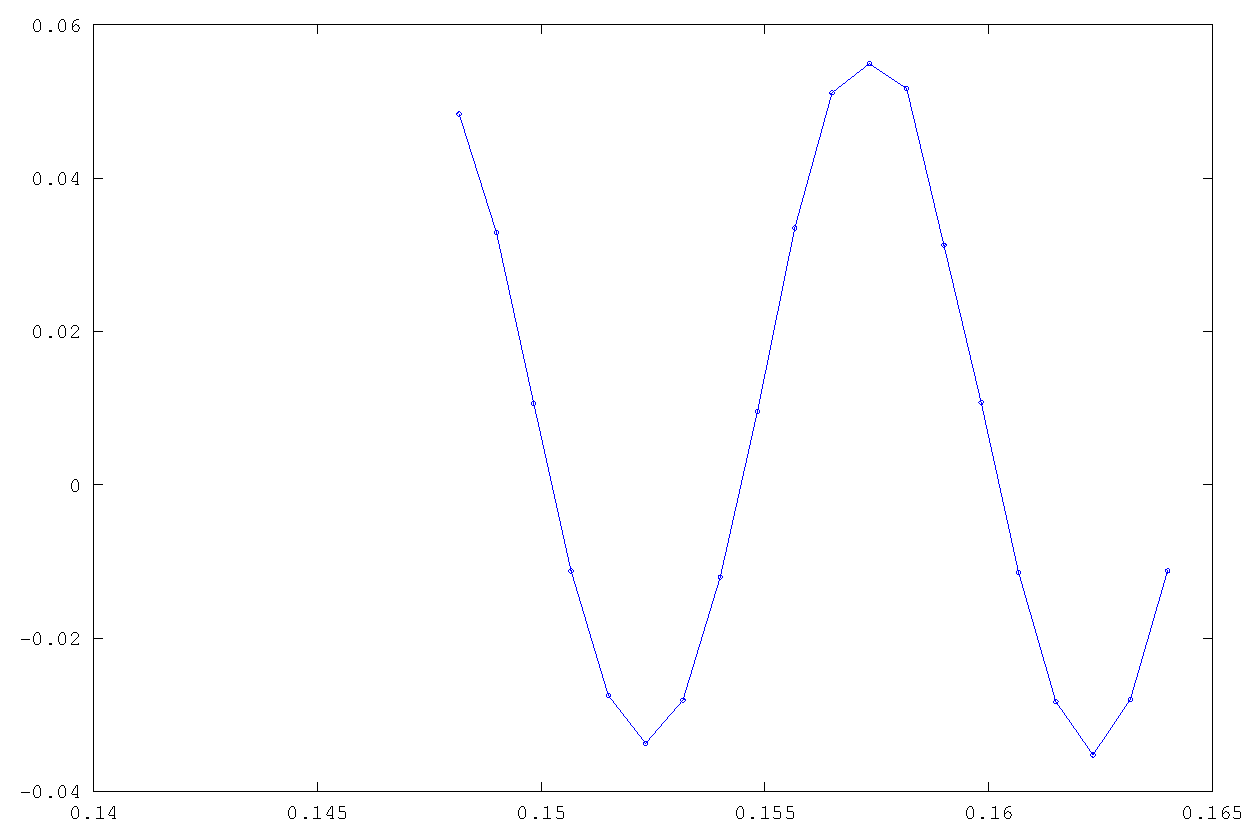
\includegraphics[width=\linewidth]{pt4_2}
	\end{center}
	\caption{Small Bins Quantization Error}
	\label{fig:smallQ}
\end{figure}

Finally we make the range covered by the quantization to large. In this case we
increase the input range from $0.1\dem{V}$ peak-to-peak to $1\dem{v}$. While it
is difficult to visualize. Compare \figref{bigQ} to \figref{4korig}. Notice the
scale of \figref{bigQ} is smaller - as if the graph was "zoomed out".
Practically this has the side affect of minimizing details in the incoming
signal that could be important for processing. 

\begin{figure}[H]
	\begin{center}
		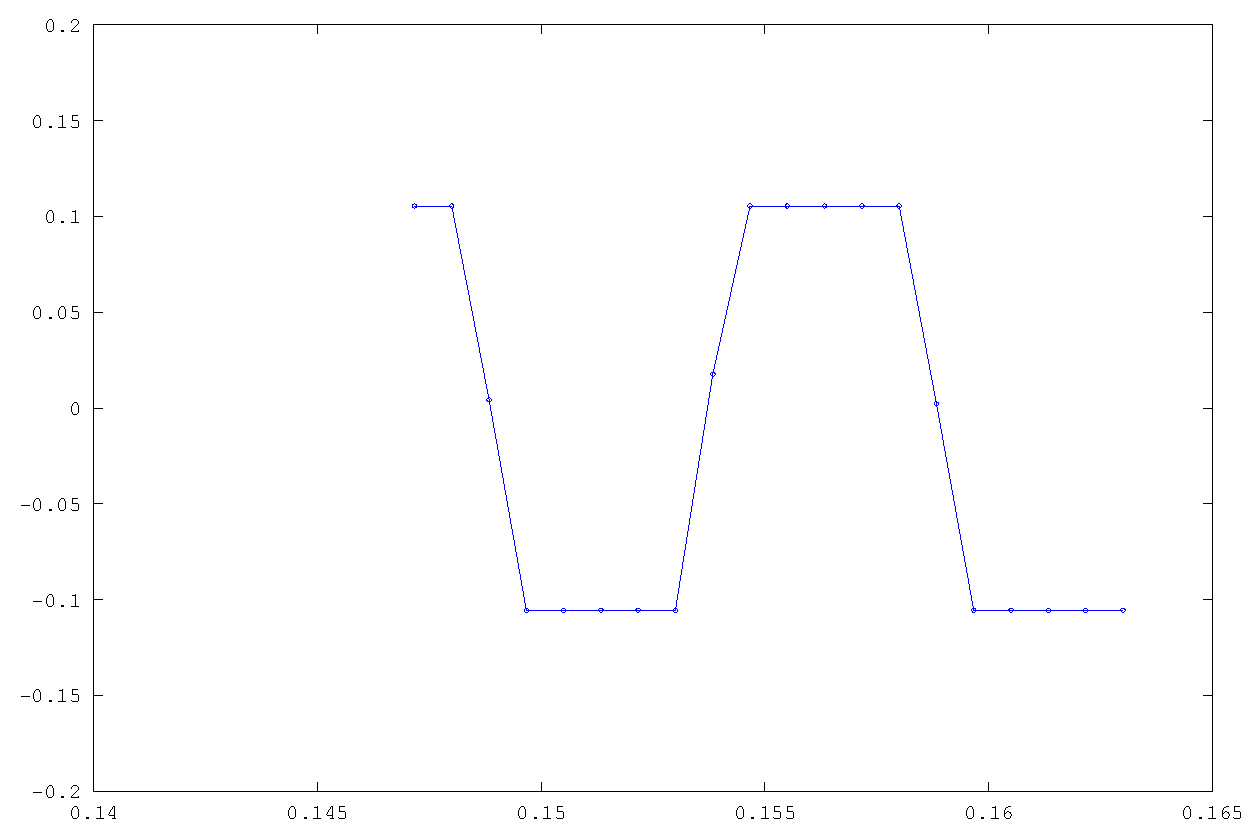
\includegraphics[width=\linewidth]{pt4_1}
	\end{center}
	\caption{Large Bins Quantization Errror}
	\label{fig:bigQ}
\end{figure}

% subsection quantization_error (end)

% subsection null_offset_error (end)

\end{document}
